\documentclass[11pt,a4paper]{article}

% --- PAQUETES PRINCIPALES ---
\usepackage[spanish,es-nodecimaldot]{babel}
\usepackage[utf8]{inputenc}
\usepackage[T1]{fontenc}
\usepackage{geometry}
\geometry{top=2.5cm, bottom=2.5cm, left=2.5cm, right=2.5cm}

\usepackage{placeins}
\usepackage{amsmath,amssymb}
\usepackage{graphicx}
\usepackage{hyperref}
\usepackage{cite}
\usepackage{microtype}

% Configuración de hipervínculos
\hypersetup{
    colorlinks=true,
    linkcolor=blue,
    filecolor=magenta,      
    urlcolor=blue,
    citecolor=blue
}

% --- DATOS DEL DOCUMENTO ---
\title{\textbf{Reporte de desarrollo del proyecto 2: Reproductor MP3 con Base de Datos e Interfaz Gráfica}}

\author{\textbf{Gómez Ferro Ana Luisa} \\
Materia: Modelado y Programación}
\date{\today}

\begin{document}

\maketitle

\begin{abstract}
En este proyecto se aborda el diseño y la implementación de un sistema en C++ para crear, consultar y manipular una base de datos musical a partir del recorrido de directorios con archivos MP3 que contienen etiquetas ID3v2. El sistema se organiza mediante programación orientada a objetos y el patrón Modelo-Vista-Controlador (MVC), apoyándose en TagLib para extraer metadatos, SQLite3 para la persistencia de datos, Google Test (GTest) para pruebas unitarias y CMake/Make para la compilación con G++. Como resultado, se obtiene un ejecutable con interfaz gráfica que permite visualizar canciones, álbumes y artistas, agregar y modificar información, realizar búsquedas y reproducir archivos MP3.
\end{abstract}

\section{Introducción}
El siguiente proyecto tiene como objetivo principal diseñar e implementar un reproductor MP3 con base de datos e interfaz gráfica utilizando el lenguaje C++ bajo el paradigma orientado a objetos, mediante la metodología del modelo en cascada (que abarca las fases de análisis, diseño, implementación, pruebas y mantenimiento, centrándonos principalmente en las etapas de análisis, diseño e implementación).
El problema central radica en brindar una interfaz gráfica intuitiva donde se visualicen los datos asociados a los archivos MP3, los álbumes y los intérpretes (performers). A través de ella, el usuario debe poder indicar directorios para poblar la base de datos, modificar la información almacenada, registrar nuevos artistas o grupos y realizar búsquedas avanzadas mediante filtros. Asimismo, el sistema debe garantizar la persistencia de los datos agregados o modificados por el usuario, manteniendo la coherencia entre la información registrada y la vista de las canciones, álbumes e intérpretes.
Durante el desarrollo se presentaron diversas dificultades, entre ellos, el estructurar correctamente el programa siguiendo el patrón MVC, diseñar un analizador de consultas capaz de manejar múltiples criterios y casos especiales (como paréntesis en títulos o filtros negativos), y garantizar la correcta persistencia y actualización de las modificaciones hechas en la base de datos.
Entre las facilidades del proyecto destacan el uso de la programación orientada a objetos para organizar los componentes del sistema, el uso del patrón de diseño DAO para comunicarse con la base de datos, y el apoyo del entorno de desarrollo para construir la interfaz gráfica.

\section{Análisis y Diseño}
El planteamiento del problema a resolver es el siguiente: se requiere un reproductor MP3 con persistencia e interfaz gráfica que se componga de cuatro componentes principales: una base de datos en SQLite3, un minero capaz de recorrer directorios y extraer metadatos de archivos MP3 (etiquetas ID3v2.4 y carátulas) para poblar la base de datos, una interfaz gráfica que permita visualizar y modificar ciertos datos almacenados, y un analizador de búsquedas que permita filtrar la información sin que el usuario tenga que escribir consultas SQL directamente. Al tratarse de la gestión y consulta estructurada de datos y archivos locales, es un problema bien definido y computable.
Para comprender y abordar el problema de manera ordenada, se divide en subproblemas: la extracción y procesamiento de archivos MP3, el almacenamiento y consulta persistente en la base de datos, la traducción de filtros de búsqueda y la presentación/interacción mediante la interfaz gráfica. A partir de esta descomposición natural dada por la especificación del problema, el diseño define cómo interactúan los componentes bajo el patrón MVC (Model-View-Controller) y el patrón DAO (Data Access Object).

\section{Diseño del Programa}
Para estructurar el sistema de manera escalable y fácil de mantener, el diseño se fundamenta en la combinación de dos patrones de diseño: Modelo-Vista-Controlador (MVC) y Data Access Object (DAO). Esta separación permite aislar la interfaz gráfica de la lógica de procesamiento y del acceso directo a la base de datos en SQLite3.

\subsection{Arquitectura General y Diagrama de Clases} 
La estructura del sistema y las relaciones entre sus componentes se muestran en la Figura~\ref{fig:diagrama_clases}. 

\begin{figure}[htbp]
    \centering
    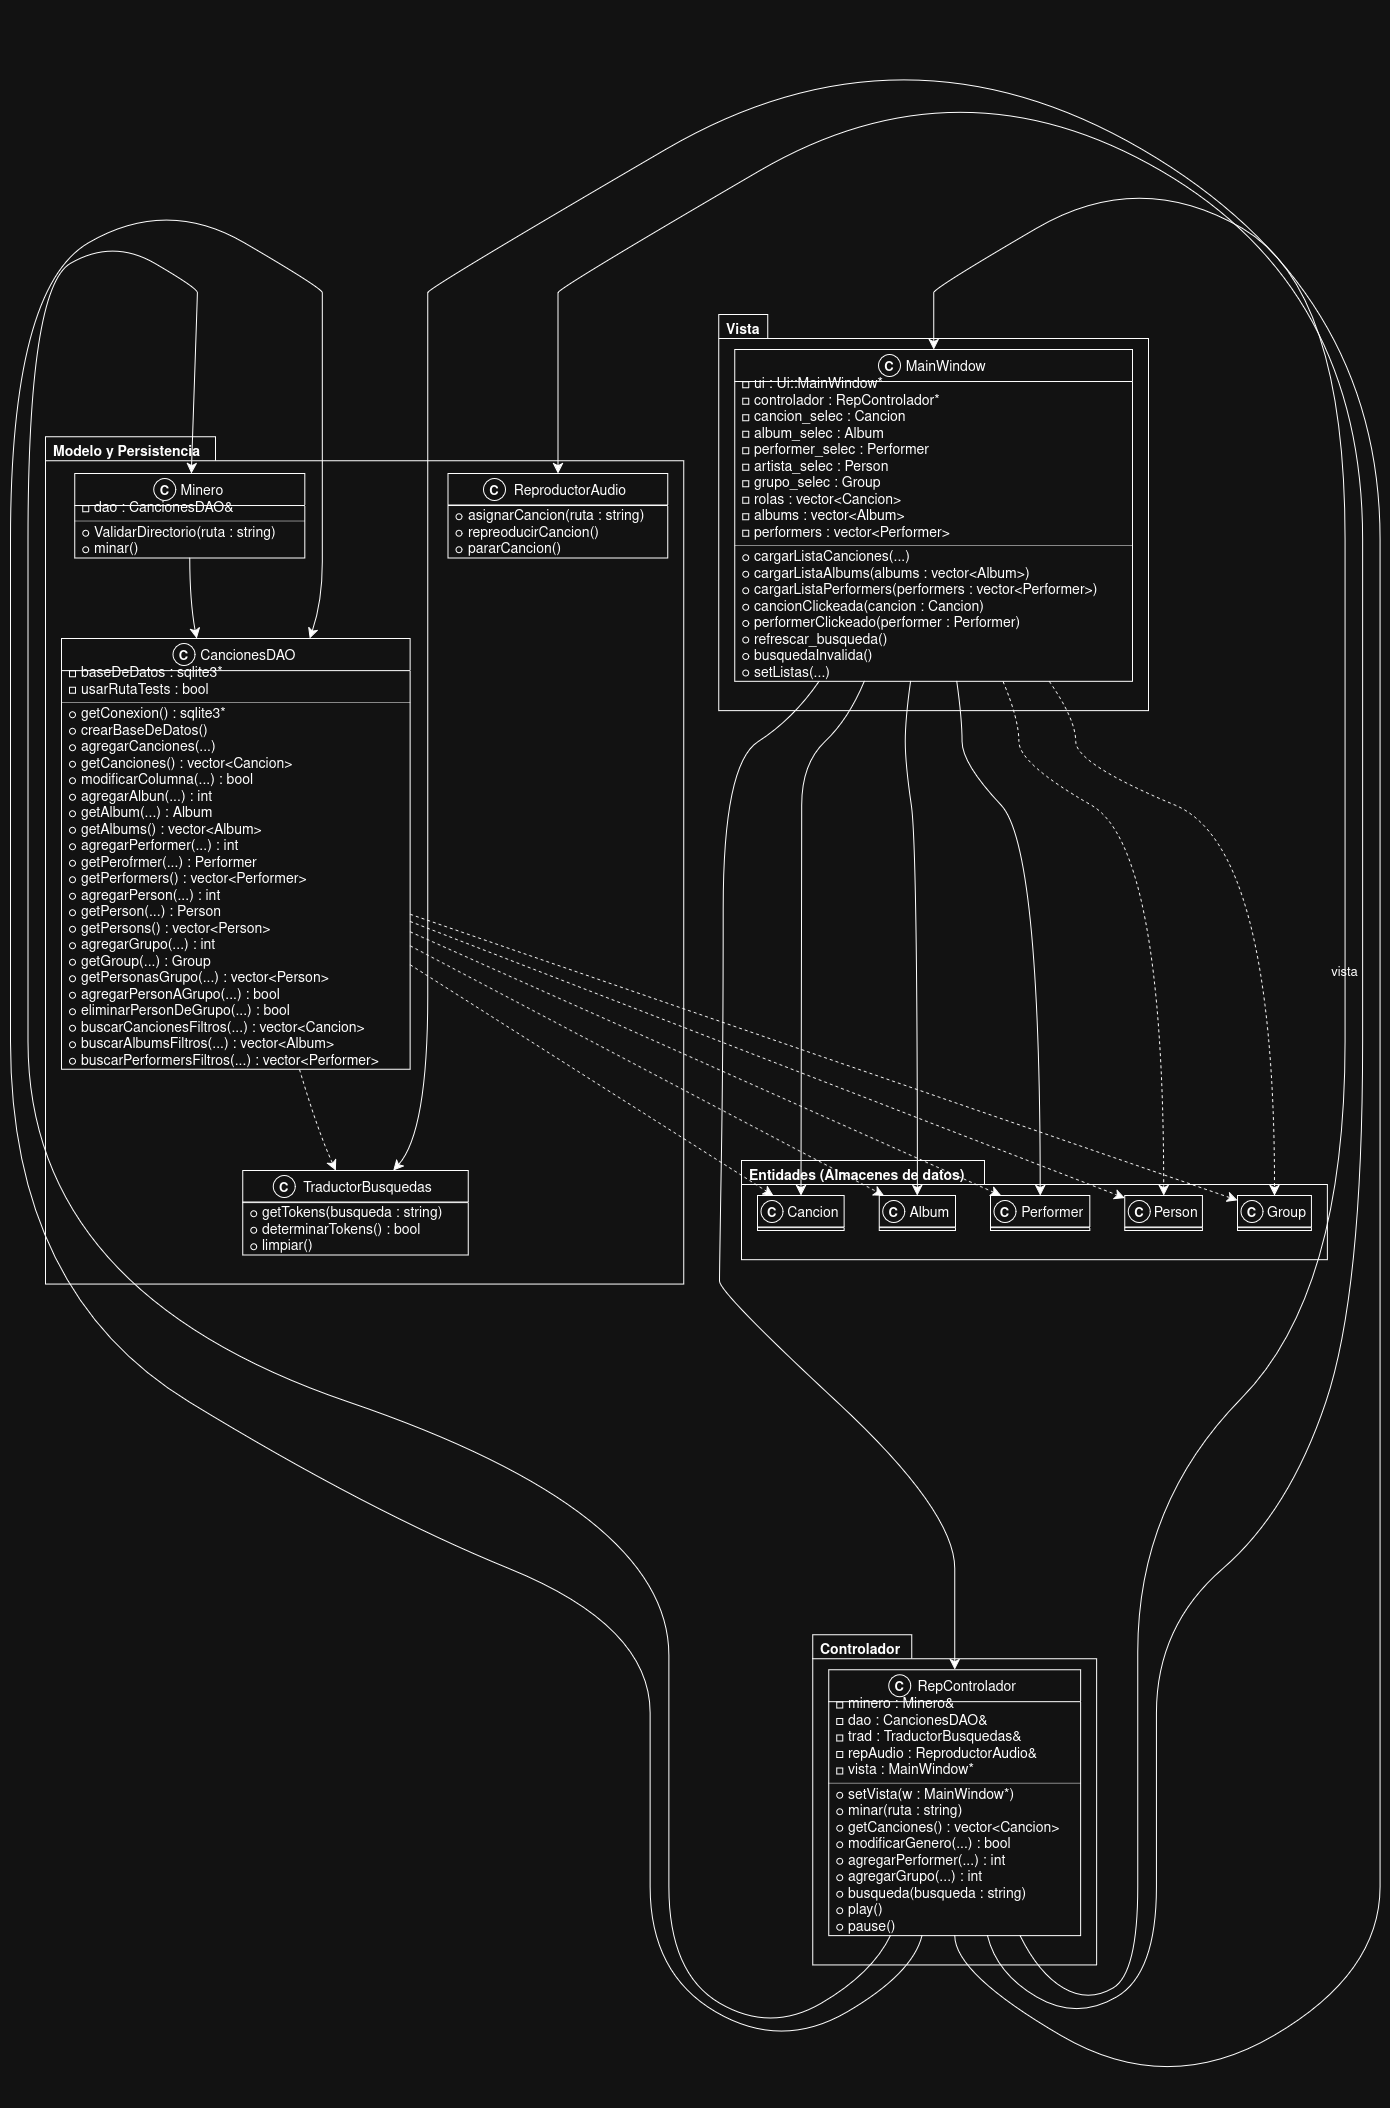
\includegraphics[width=0.95\textwidth]{imagenes/Diagrama_clases.drawio.png}
    \caption{Diagrama de clases del reproductor MP3 bajo la arquitectura MVC y el patrón DAO.}
    \label{fig:diagrama_clases}
\end{figure}

Desde la función principal (\texttt{main}) se instancian e inyectan las dependencias principales del sistema:

\begin{itemize}
    \item \textbf{Modelo:} Está conformado por \texttt{CancionesDAO}, encargada de crear la base de datos, ejecutar consultas SQL y modificar registros en SQLite3 devolviendo estructuras de datos, \texttt{Minero}, responsable de recorrer directorios, validar archivos MP3, extraer etiquetas ID3v2.4 y guardar carátulas, \texttt{TraductorBusquedas}, encargado de analizar y validar las cadenas de búsqueda ingresadas por el usuario, y \texttt{ReproductorAudio}, que gestiona la reproducción multimedia.
    
    \item \textbf{Estructuras de Datos:} Las estructuras \texttt{Cancion}, \texttt{Album}, \texttt{Performer}, \texttt{Person} y \texttt{Group} funcionan únicamente como contenedores de información para transportar datos entre clases.

    \item \textbf{Controlador:} Representada por \texttt{RepControlador}, coordina la interacción entre la vista y el modelo, delegando la mayoría de las operaciones directamente a métodos de \texttt{CancionesDAO}, \texttt{Minero} o \texttt{ReproductorAudio}.
    
    \item \textbf{Vista:} Implementada en \texttt{MainWindow} (junto con diálogos secundarios \texttt{QDialog}), se encarga de presentar la información al usuario, capturar sus eventos y solicitar las acciones correspondientes al controlador.
    \end{itemize}

    \subsection{Flujo de Búsquedas Avanzadas} 
    A diferencia de las operaciones simples de consulta o edición (donde la vista solicita una acción al controlador y posteriormente refresca los datos), el proceso de búsqueda requiere coordinar múltiples componentes. Como se ilustra en la Figura~\ref{fig:secuencia_busqueda}, cuando el usuario ingresa una búsqueda con filtros, \texttt{RepControlador::busqueda()} envía la cadena a \texttt{TraductorBusquedas} para generar y validar los \textit{tokens}. Si la expresión es válida, el controlador solicita a \texttt{CancionesDAO} las coincidencias filtradas de canciones, álbumes e intérpretes, actualiza las listas en \texttt{MainWindow} y ordena refrescar la interfaz. En caso contrario, notifica a la vista que la consulta es inválida. 
    
    \begin{figure}[htbp] 
    \centering 
    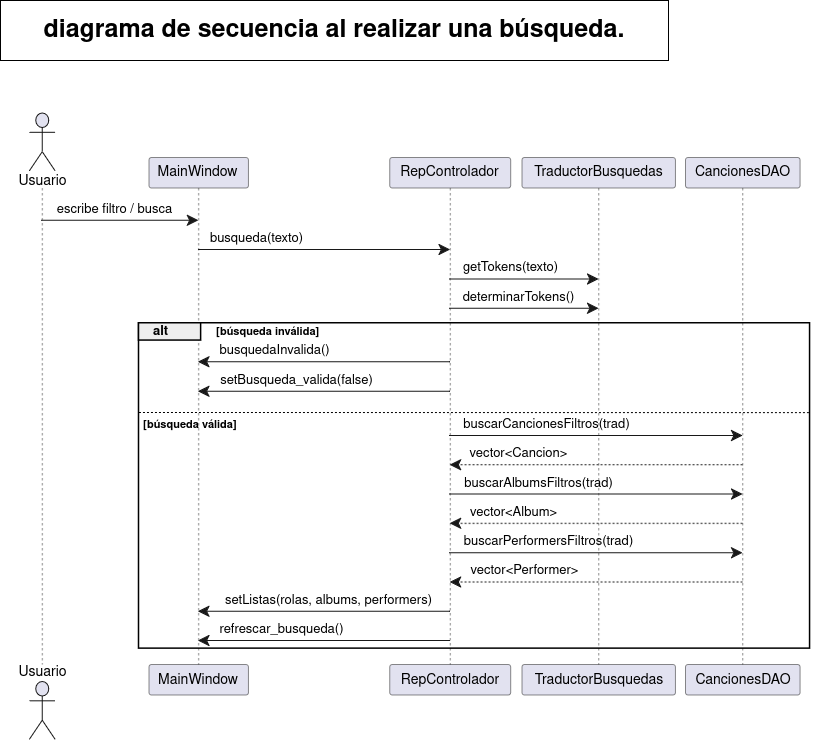
\includegraphics[width=0.95\textwidth]{imagenes/Diagrama_secuencia_busqueda.drawio.png} 
    \caption{Diagrama de secuencia para el procesamiento y filtrado de búsquedas.} \label{fig:secuencia_busqueda} 
    \end{figure}


    \subsection{Diseño de la Interfaz Gráfica} 
    La interfaz gráfica fue desarrollada en Qt combinando el entorno visual de Qt Creator (mediante archivos \texttt{.ui}) con hojas de estilo (QSS). La lógica fue escrita en C++ (\texttt{.h} y \texttt{.cpp}) y se usaron contenedores dinámicos (\texttt{QStackedWidget}) para alternar entre las distintas vistas de navegación y edición sin saturar la pantalla principal, además de ventanas emergentes basadas en \texttt{QDialog} para los diálogos de edición.

    En las Figuras ~\ref{fig:vista_canciones},~\ref{fig:vista_albums}, ~\ref{fig:vista_artistas} se presentan las vistas principales del reproductor, donde se visualizan los listados de canciones, álbumes o intérpretes junto con los controles de reproducción, edición y la barra de búsqueda. 
    Por su parte, las Figuras~\ref{fig:editar_album} y ~\ref{fig:editar_integrantes} muestran el diálogo de edición de metadatos en los álbumes, y el diálogo para añadir integrantes a los grupos (los demás diálogos del sistema siguen una estructura y dinámica similares). 

    \begin{figure}[htbp] 
    \centering 
    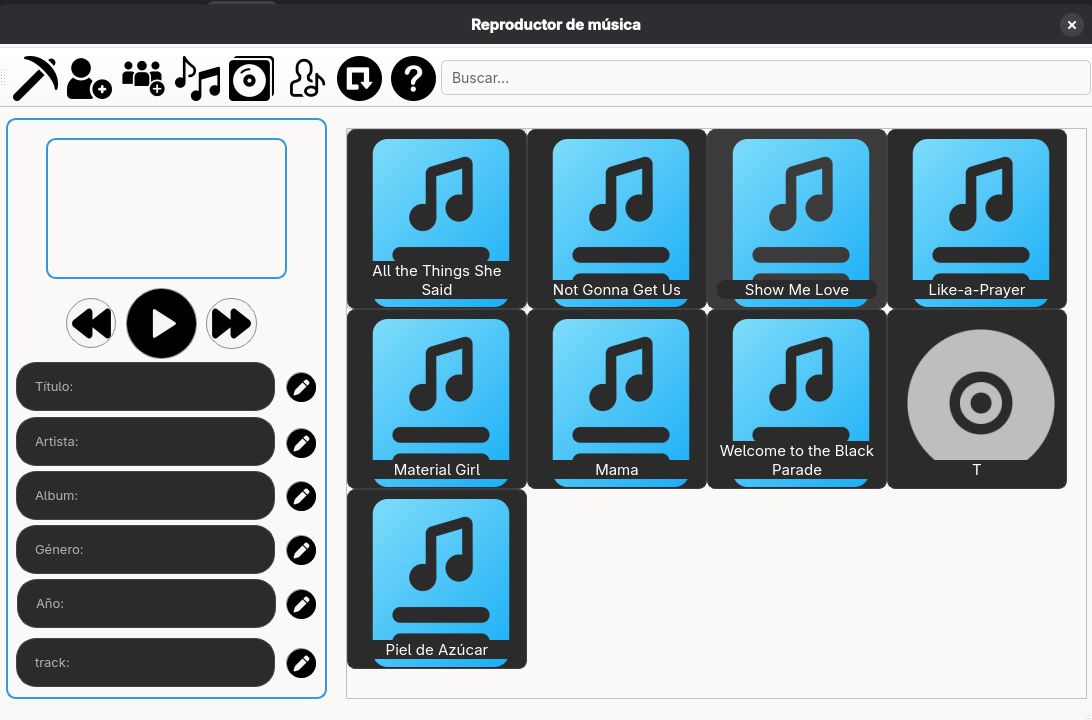
\includegraphics[width=0.9\textwidth]{imagenes/vista_canciones.png} 
    \caption{Vista de canciones.} \label{fig:vista_canciones} \end{figure} 

    \begin{figure}[htbp] 
    \centering 
    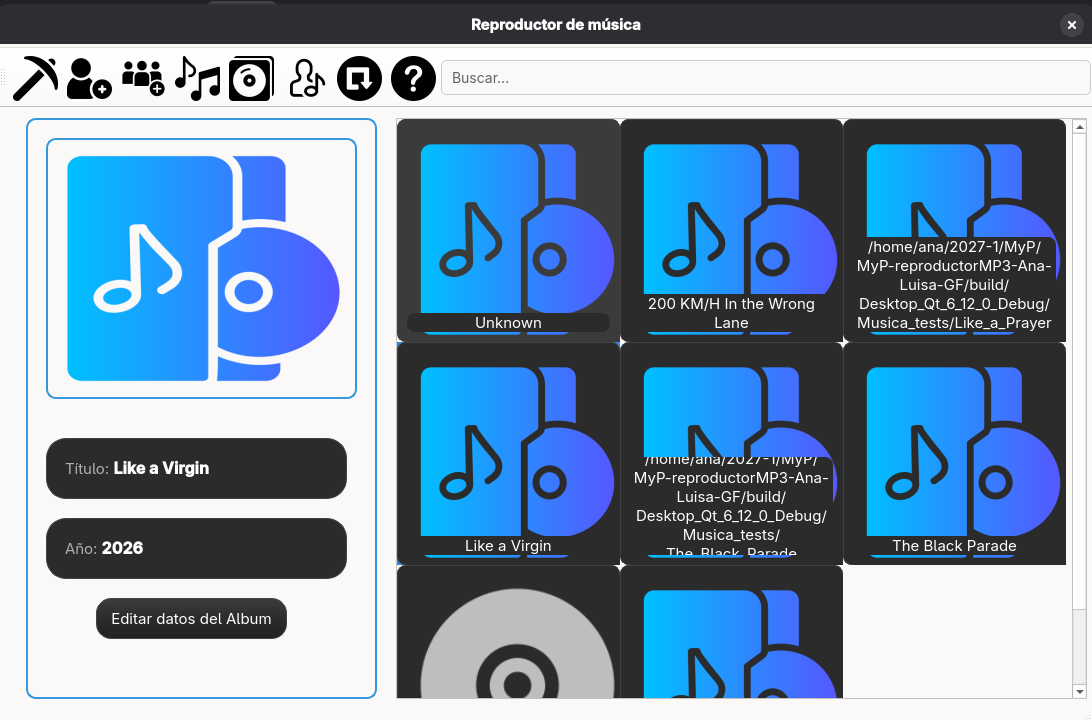
\includegraphics[width=0.9\textwidth]{imagenes/vista_albums.png} 
    \caption{Vista de álbumes.} \label{fig:vista_albums}
    \end{figure} 

    \begin{figure}[htbp] 
    \centering 
    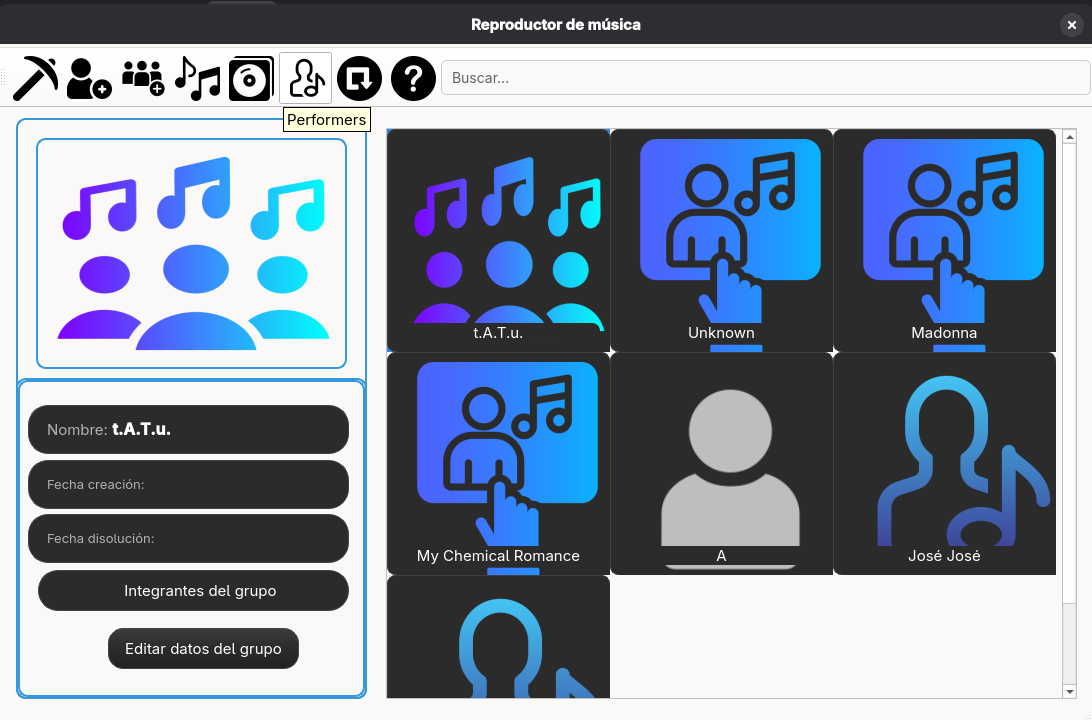
\includegraphics[width=0.9\textwidth]{imagenes/vista_artistas.png} 
    \caption{Vista de artistas.} \label{fig:vista_artistas}
    \end{figure} 

    \begin{figure}[htbp] 
    \centering 
    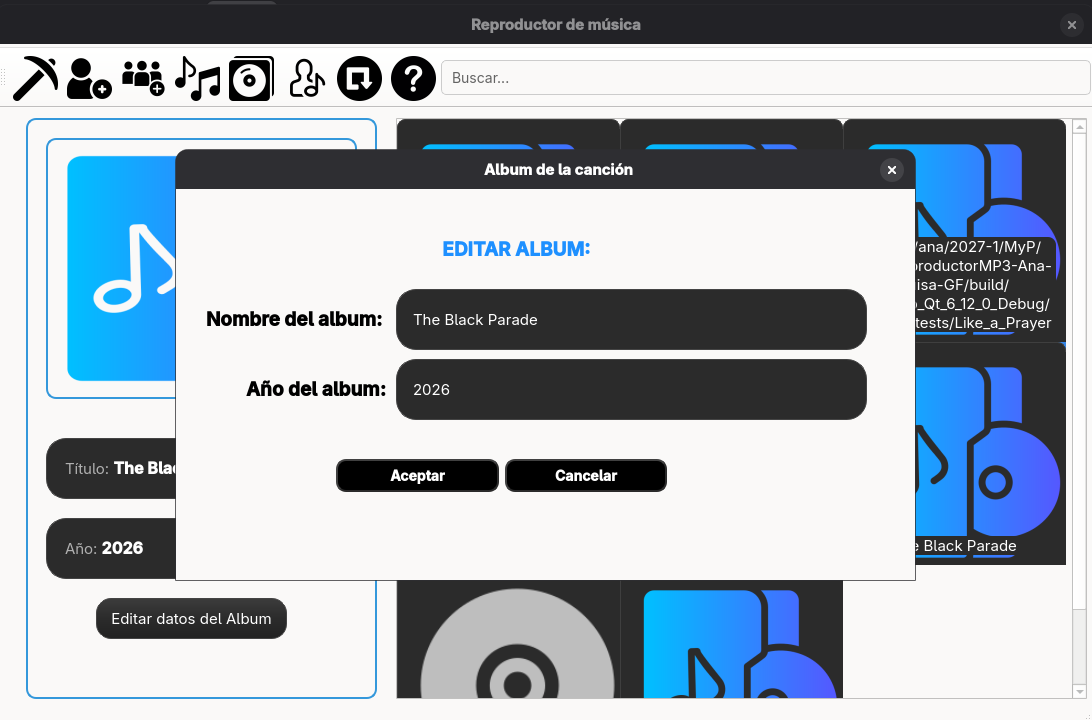
\includegraphics[width=0.9\textwidth]{imagenes/editar_album.png} 
    \caption{Vista de el diálogo de edición de datos para los álbumes} \label{fig:editar_album}
    \end{figure} 

    \begin{figure}[htbp] 
    \centering 
    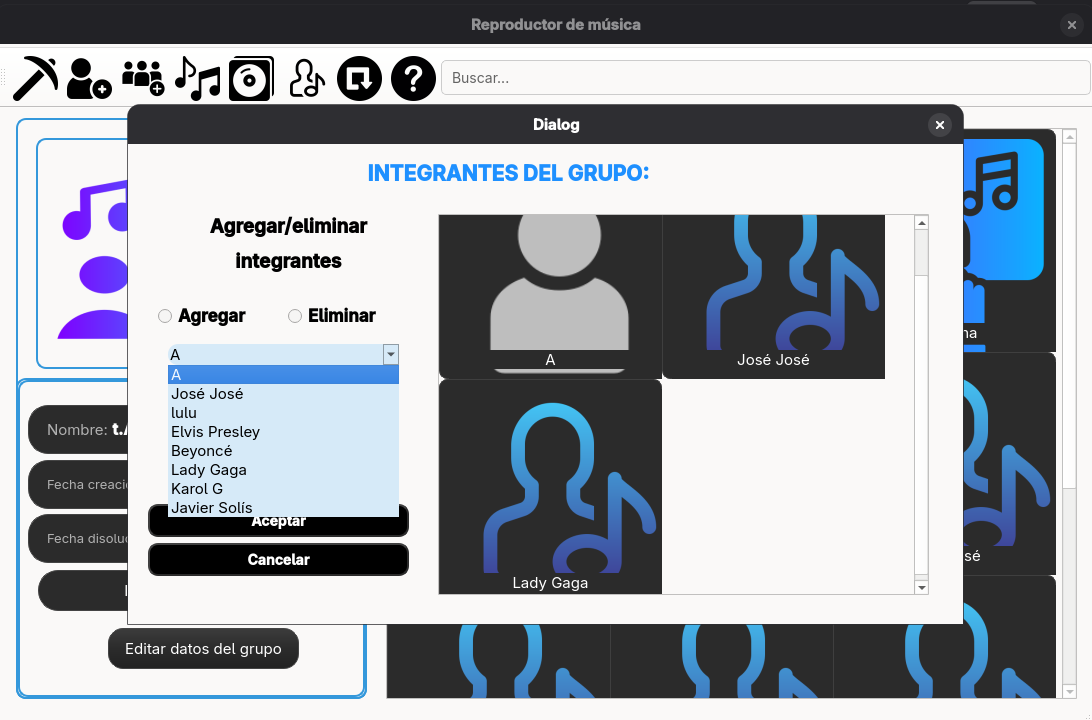
\includegraphics[width=0.9\textwidth]{imagenes/editar_integrantes.png} 
    \caption{Vista de el diálogo para insertar artistas como integrantes de un grupo.} \label{fig:editar_integrantes}
    \end{figure} 

    \FloatBarrier
        \subsection{Alternativas Consideradas y Evolución del Diseño}
    Antes de llegar al diseño actual, se evaluaron otras alternativas que resultaron poco prácticas o desordenadas conforme el programa fue creciendo. Al principio se consideró un enfoque más directo y centralizado, concentrando lectura de archivos, consultas y manejo de la interfaz en un mismo flujo para avanzar rápido; sin embargo, esto habría hecho el código difícil de mantener al incorporar búsquedas con filtros o edición de datos. Combinar MVC y DAO permitió separar mejor las responsabilidades: \texttt{CancionesDAO} concentra la persistencia en SQLite3, \texttt{RepControlador} coordina las acciones y \texttt{MainWindow} se encarga de la interfaz y los eventos del usuario.
    
    A lo largo del desarrollo también surgieron varios tropiezos y ajustes sobre la marcha:
    \begin{itemize}
    \item \textbf{Curva de aprendizaje y rediseños de la interfaz:} Adaptarme a Qt llevó tiempo, por lo que las primeras versiones tenían una presentación muy básica: listas simples, sin carátulas en las canciones y sin secciones como la de álbumes. A medida que fui dominando la herramienta y combinando los archivos \texttt{.ui}, las hojas de estilo (QSS) y la lógica en C++, rediseñé la interfaz en varias ocasiones para hacerla más clara y amigable.
    
    \item \textbf{Ajustes en el minero:} Al inicio no contemplaba extraer ni mostrar carátulas de los archivos MP3, pero durante el desarrollo se amplió \texttt{Minero} para guardar las portadas.
    
    \item \textbf{Búsquedas y consistencia de datos:} Implementar \texttt{TraductorBusquedas} para manejar filtros, negativos o paréntesis, así como asegurar que las modificaciones de la interfaz se guardaran y refrescaran correctamente en SQLite3, requirió varias iteraciones y pruebas entre componentes.
    \item \textbf{Consultas SQL:} Me costó trabajo entender bien cómo armar las consultas en SQLite3 y solía cometer varios errores al redactarlas, ya fuera por detalles de sintaxis, nombres de variables o índices al leer columnas, especialmente al construir búsquedas con filtros y parámetros.
    \end{itemize}
    
    \section{Implementación}
    
    Para el desarrollo del sistema se utilizó C++17 como lenguaje de programación, aprovechando el paradigma orientado a objetos para organizar las clases y estructuras del reproductor. Para la interfaz gráfica y la reproducción de audio se empleó Qt6 (con sus módulos de \textit{Widgets} y \textit{Multimedia}), mientras que la lectura de metadatos y carátulas de archivos MP3 se apoyó en TagLib, y la persistencia local se gestionó mediante SQLite3. En la infraestructura de construcción se utilizaron CMake (versión 3.12 o superior) y Make junto con el compilador \texttt{g++}, ademas de Google Test (GTest) para las pruebas unitarias.
    
    Para preparar el entorno y compilar el proyecto desde la raíz, se ejecutan los comandos \texttt{cmake -B build} y posteriormente \texttt{cmake --build build}, generando los binarios dentro del directorio \texttt{build}. Las pruebas unitarias pueden ejecutarse de forma individual mediante \texttt{./build/test\_CancionesDAO} y \texttt{./build/test\_Minero}, y la aplicación principal se inicia con el ejecutable \texttt{./build/Reproductor}.
    
    \section{Conclusiones}
    
    El desarrollo de este proyecto representó un aprendizaje integral sobre cómo estructurar y construir una aplicación de escritorio completa en C++ con interfaz gráfica y persistencia de datos. A lo largo del proceso aprendí a integrar distintas herramientas y bibliotecas (como Qt6 para la interfaz y la reproducción multimedia, TagLib para la extracción de metadatos ID3v2.4 y SQLite3 para el almacenamiento local) dentro de un mismo sistema organizado con CMake. Uno de los aspectos más desafiantes fue visualizar desde las primeras etapas cómo debían comunicarse todas las capas del programa y diseñar el analizador de búsquedas (\texttt{TraductorBusquedas}) junto con las consultas SQL dinámicas para filtrar información.
    
    Durante la implementación identifiqué decisiones de diseño que pude haber resuelto mejor desde el principio. Por ejemplo, al inicio llegué a mezclar responsabilidades relacionadas con la base de datos dentro de \texttt{Minero}, hasta que reubiqué toda la creación de tablas y operaciones exclusivamente en \texttt{CancionesDAO} para mantener una separación limpia entre la extracción de archivos y la base de datos. De manera similar, los primeros diseños de la interfaz gráfica fueron demasiado básicos por la curva de aprendizaje con Qt, lo que obligó a rediseñar varias vistas y diálogos sobre la marcha. Además, una mejor gestión del tiempo habría permitido ampliar la cobertura de pruebas unitarias hacia el controlador y el traductor de búsquedas, así como incorporar funciones adicionales en el reproductor.
    
    Finalmente, comprobé en la práctica el valor de aplicar patrones de diseño como Modelo-Vista-Controlador (MVC) y Data Access Object (DAO), los cuales facilitaron ordenar el código, aislar el acceso a SQLite3 y evolucionar la interfaz gráfica sin tener que reescribir la lógica central. Como trabajo a futuro, la arquitectura actual permitiría extender el sistema para incorporar listas de reproducción personalizadas, búsquedas mas avanzadas, mas opciones respecto al audio (como tener una barra de reproducción o control del volumen), etc.

    \section{Bibliografía}
    
    \subsection{Documentación y Recursos Técnicos}
    \begin{itemize}
        \item The Qt Company. \textit{Qt Creator Manual}. \url{https://doc.qt.io/qtcreator/}
        \item The Qt Company. \textit{QMediaPlayer Class | Qt Multimedia 6}. \url{https://doc.qt.io/qt-6/qmediaplayer.html}
        \item TagLib Developers. \textit{TagLib API Reference}. \url{https://taglib.org/api/}
        \item Qt Wiki. \textit{Qt for Beginners}. \url{https://wiki-qt-io.translate.goog/Qt_for_Beginners?_x_tr_sl=en&_x_tr_tl=es&_x_tr_hl=es&_x_tr_pto=tc}
        \item freeCodeCamp. \textit{Learn SQL Queries --- Database Query Tutorial for Beginners}. \url{https://www-freecodecamp-org.translate.goog/news/learn-sql-queries-database-query-tutorial-for-beginners/?_x_tr_sl=en&_x_tr_tl=es&_x_tr_hl=es&_x_tr_pto=tc}
        \item IONOS. \textit{SQL Joins: explicación y ejemplos}. \url{https://www.ionos.mx/digitalguide/servidores/configuracion/sql-joins/}
        \item Lista de reproducción de consulta en YouTube (1). \url{https://youtube.com/playlist?list=PL54fdmMKYUJvn4dAvziRopztp47tBRNum&si=Q1GuZAujNSu-IFPB}
        \item Lista de reproducción de consulta en YouTube (2). \url{https://youtube.com/playlist?list=PLZgahc8X4J81ey9cvShF5bNEjC8kDzVVD&si=YyTOaCIr6UKSfm0G}
    \end{itemize}
    
    \subsection{Íconos e Imágenes Utilizadas}
    Todos los íconos de la interfaz se obtuvieron de Flaticon bajo sus respectivas atribuciones de autoría:
    \begin{itemize}
        \item \textbf{Botón de play:} Creado por Alfredo Hernandez en Flaticon. \url{https://www.flaticon.es/iconos-gratis/boton-de-play}
        \item \textbf{Botón de pausa:} Creado por SumberRejeki en Flaticon. \url{https://www.flaticon.es/iconos-gratis/boton-de-pausa}
        \item \textbf{Botón siguiente:} Creado por adrianadam en Flaticon. \url{https://www.flaticon.es/iconos-gratis/siguiente}
        \item \textbf{Botón atrás:} Creado por Erix en Flaticon. \url{https://www.flaticon.es/iconos-gratis/interfaz-de-usuario}
        \item \textbf{Minar:} Creado por Magnific en Flaticon. \url{https://www.flaticon.es/iconos-gratis/pico}
        \item \textbf{Sección de canciones:} Creado por Magnific en Flaticon. \url{https://www.flaticon.es/iconos-gratis/musica}
        \item \textbf{Reproductor de música base:} Creado por Icon Place en Flaticon. \url{https://www.flaticon.es/iconos-gratis/google-play-music}
        \item \textbf{Álbum base:} Creado por Mayor Icons en Flaticon. \url{https://www.flaticon.es/iconos-gratis/album-de-musica}
        \item \textbf{Grupo base:} Creado por afif fudin en Flaticon. \url{https://www.flaticon.es/iconos-gratis/musico}
        \item \textbf{Performer base:} Creado por nangicon en Flaticon. \url{https://www.flaticon.es/iconos-gratis/artista}
        \item \textbf{Artista base:} Creado por th studio en Flaticon. \url{https://www.flaticon.es/iconos-gratis/artista}
        \item \textbf{Agregar artista:} Creado por uicon en Flaticon. \url{https://www.flaticon.es/iconos-gratis/agregar-usuario}
        \item \textbf{Agregar grupo:} Creado por siens en Flaticon. \url{https://www.flaticon.es/iconos-gratis/anadir-grupo}
        \item \textbf{Ayuda:} Creado por Magnific en Flaticon. \url{https://www.flaticon.es/iconos-gratis/pregunta}
        \item \textbf{Actualizar:} Creado por Laisa Islam Ani en Flaticon. \url{https://www.flaticon.es/iconos-gratis/rechazar}
\end{itemize}
\end{document}
